\documentclass{beamer}
\usepackage{graphicx}
\usepackage{minted}
\graphicspath{ {./} }
\usepackage{minted}
\floatname{listing}{Code snippet}

\usetheme{Madrid}

\title{Moon rover simulation with RabbitMQ communication}

\author{Papp Gellért-Szabolcs}

\date{\ }

\begin{document}
    
\maketitle

\begin{frame}{The project}
    \begin{itemize}
        \item An unrealistic simulation of a moon rover
        \item The moon rover communicates with a server
        \item Clients can view the current state of the moon rover and they can "control" it by connecting to the server
        \item Command line only
    \end{itemize}
\end{frame}

\begin{frame}{Architecture}
    The project has the following architecture:

    \ 

    \begin{figure}
        \centering
        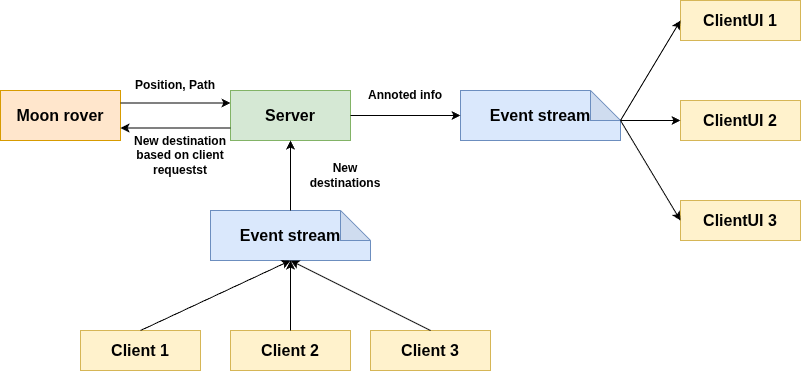
\includegraphics[width=0.90\linewidth]{architecture.png}
    \end{figure}
\end{frame}

\begin{frame}{Communication}
    \begin{itemize}
        \item The communication happens with RabbitMQ streams
        \item This is because streams allow for better communication with multiple clients at the same time
        \item It also allows the server to do work based on the timestamp of messages
        \item Note: The server to moon rover communication could simply be done with queues 
    \end{itemize}
\end{frame}

\begin{frame}{Moon rover}
    \begin{itemize}
        \item The "moon rover" is placed on a square region on the "moon"
        \item It receives commands from the server on Earth; the commands tell it what region of the moon it should move to
        \item The rover chooses the shortest path from its current location to its next destination
        \item As it moves along, it sends signals about its whereabouts and its planned path to the server
    \end{itemize}
\end{frame}

\begin{frame}{Server}
    \begin{itemize}
        \item The server parses the moon rover data and sends events to a stream that can be read by the clients
        \item From time to time, it also looks at new destination suggestions made by the clients in a time interval and sends a final new destination to the moon rover
    \end{itemize}
\end{frame}

\begin{frame}{Clients}
    There are two kinds of clients.
    \begin{itemize}
        \item Clients that visualize the position of the rover
        \item Clients that vote on the next destination of the rover
    \end{itemize}
\end{frame}

\begin{frame}{Sample code: Producer}
    \inputminted[ 
        breaklines,
        fontsize=\tiny,
    ]{rust}{prod.rs}
\end{frame}

\begin{frame}{Sample code: Consumer}
    \inputminted[ 
        breaklines,
        fontsize=\tiny,
    ]{rust}{cons.rs}
\end{frame}

\begin{frame}{I'm done (with the presentation, we still have the demo)}
    \begin{figure}
        \centering
        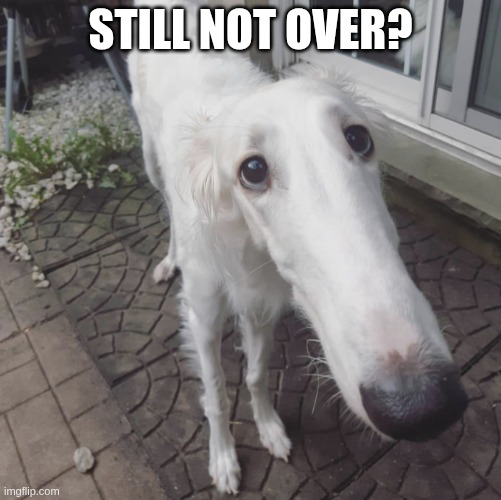
\includegraphics[width=0.60\linewidth]{end_it.png}
    \end{figure}
\end{frame}

\end{document}
